\documentclass{bioinfo}
\copyrightyear{2013}
\pubyear{2013}
%\usepackage[top=1in, bottom=1in,right=1in,left=1in]{geometry}                % See geometry.pdf to learn the layout options. There are lots.
%\geometry{letterpaper}                   % ... or a4paper or a5paper or ... 
%\geometry{landscape}                % Activate for for rotated page geometry
%\usepackage[parfill]{parskip}    % Activate to begin paragraphs with an empty line rather than an indent
%\usepackage[utf8]{inputenc}
\usepackage{graphicx}
\usepackage{amssymb}
\usepackage{amsmath}
\usepackage{amsthm} %pour les newtheorem
\usepackage{epstopdf}
\usepackage{framed}
\usepackage{xspace}
%\usepackage{tcolorbox}
\usepackage{relsize}
%\usepackage{natbib}
\usepackage[colorinlistoftodos]{todonotes}

\usepackage{soul}

\colorlet{shadecolor}{yellow!80!orange!50}
\sethlcolor{shadecolor}
\makeatletter

\renewenvironment{snugshade}{%
 \def\FrameCommand##1{\hskip\@totalleftmargin \hskip-\fboxsep
 \colorbox{shadecolor}{##1}\hskip-\fboxsep
     % There is no \@totalrightmargin, so:
     \hskip-\linewidth \hskip-\@totalleftmargin \hskip\columnwidth}%
 \MakeFramed {\advance\hsize-\width
   \@totalleftmargin\z@ \linewidth\hsize
   \@setminipage}}%
 {\par\unskip\endMakeFramed}

\makeatother

\newcommand{\highlight}[1]{{\begin{snugshade}{#1}\end{snugshade}}}

%\usepackage{subfig} %Subfigures
\usepackage{subcaption} %Subfigures

\usepackage{tikz}
\usepackage{amsmath}
\usepackage{ifthen}
\usepackage{relsize}
\usepackage{multirow}
\usepackage{cleveref}
\usepackage{url}

\usetikzlibrary{positioning}
\usetikzlibrary{matrix}
\usetikzlibrary{calc}
\usetikzlibrary{shapes}
\usetikzlibrary{arrows}
\usetikzlibrary{fit}
\usetikzlibrary{decorations}
\usetikzlibrary{snakes}
\usetikzlibrary{shadows}
\pgfdeclarelayer{background}
\pgfdeclarelayer{backbackground}
\pgfdeclarelayer{foreground}
\pgfsetlayers{backbackground,background,main,foreground}

\usepackage[noend,ruled,vlined]{algorithm2e}

\newtheorem{theorem}{Theorem}[section]
\newtheorem{lemma}[theorem]{Lemma}
\newtheorem{proposition}[theorem]{Proposition}
\newtheorem{corollary}[theorem]{Corollary}
\newtheorem{description}{Description}

\crefmultiformat{equation}{Equations~(#2#1#3)}%
{ and~(#2#1#3)}{, (#2#1#3)}{ and~(#2#1#3)}



\newcommand{\RNAmutants}{\texttt{RNAmutants}\xspace}
\newcommand{\RNApyro}{\texttt{RNApyro}\xspace}
\newcommand{\RNAinverse}{\texttt{RNAinverse}\xspace}
\newcommand{\RNASSD}{\texttt{RNA-SSD}\xspace}
\newcommand{\INFORNA}{\texttt{INFO-RNA}\xspace}
\newcommand{\NUPACK}{\texttt{NUPACK:Design}\xspace}
\newcommand{\RNAiFOLD}{\texttt{RNAiFOLD}\xspace}
\newcommand{\frankenstein}{\texttt{Frnakenstein}\xspace}
\newcommand{\RNAexinv}{\texttt{RNAexinv}\xspace}
\newcommand{\rnaDesign}{\texttt{rnaDesign}\xspace}
\newcommand{\RNAensign}{\texttt{RNA-ensign}\xspace}
\newcommand{\GC}{\Gb\Cb}
\newcommand{\GCContent}{\Gb\Cb-content\xspace}
\newcommand{\SFold}{\texttt{SFold}\xspace}
\newcommand{\GCWeighted}{\Gb\Cb-weighted\xspace}


\newcommand{\ourprog}{\texttt{IncaRNAtion}\xspace} 

\newcommand{\red}[1]{{\color{red}#1}}
\newcommand{\farna}{\texttt{FARNA}\xspace}
\newcommand{\mcfoldmcsym}{\texttt{MC-Pipeline}\xspace}
\newcommand{\mcfold}{\texttt{MC-Fold}\xspace}
\newcommand{\mcsym}{\texttt{MC-Sym}\xspace}
\newcommand{\nast}{\texttt{NAST}\xspace}
\newcommand{\ifoldrna}{\texttt{iFoldRNA}\xspace}
\newcommand{\rnafold}{\texttt{RNAfold}\xspace}
\newcommand{\rnasubopt}{\texttt{RNAsubopt}\xspace}
\newcommand{\rnawolf}{\texttt{RNAwolf}\xspace}
\newcommand{\rnastructure}{\texttt{RNAstructure}\xspace}
\newcommand{\contrafold}{\texttt{contrafold}\xspace}
\newcommand{\unafold}{\texttt{unafold}\xspace}
\newcommand{\rnadd}{\texttt{RNA2D3D}\xspace}
\newcommand{\assemble}{\texttt{assemble}\xspace}
\newcommand{\fred}{\texttt{FR3D}\xspace}
\newcommand{\rnajunction}{\texttt{RNAjunction}\xspace}
\newcommand{\rnamotif}{\texttt{RNAmotif}\xspace}
\newcommand{\treefolder}{\texttt{TreeFolder}\xspace}
\newcommand{\barnacle}{\texttt{BARNACLE}\xspace}
\newcommand{\contextfold}{\texttt{contextfold}\xspace}

\newcommand{\RNASTRAND}{{\sf RNA STRAND}\xspace}

%\newcommand{\citep}{\cite}
\newcommand{\Z}[2]{\mathcal{Z}{\substack{[#2]\\#1}}}
\newcommand{\B}{\mathcal{B}}
\newcommand{\Kron}{\delta}
\newcommand{\ub}{\bullet}
\newcommand{\op}{\texttt{(}}
\newcommand{\cp}{\texttt{)}}

\newcommand{\Ab}{{\sf{A}}\xspace}
\newcommand{\Cb}{{\sf{C}}\xspace}
\newcommand{\Gb}{{\sf{G}}\xspace}
\newcommand{\Ub}{{\sf{U}}\xspace}

\newcommand{\gc}{{\#\text{{\sf gc}}}}
\newcommand{\PE}[1]{E(#1)}
\newcommand{\EI}{\text{EI}}
\newcommand{\ES}{{{E}}}
\newcommand{\ISO}{\text{ISO}}
\newcommand{\Prob}{\mathbb{P}}
\newcommand{\Target}{{S}^*}
\newcommand{\Struct}{{S}}
\newcommand{\N}{{N}}
\newcommand{\CNBP}[1]{\gamma(#1)}
\newcommand{\BoolTrue}{{\sf T}}
\newcommand{\BoolFalse}{{\sf F}}

\newcommand{\CFramed}[2][gray]{\begin{tcolorbox}[colframe=#1,title=To be included only if space allows\ldots,colback=white]#1\end{tcolorbox}}
\renewcommand{\CFramed}[2][gray]{}

\newcommand{\oururl}{\url{http://csb.cs.mcgill.ca/incarnation/}}

\begin{document}
\firstpage{1}

\title{A weighted sampling algorithm for the design of RNA sequences with targeted secondary structure and nucleotide distribution}
\author{Vladimir Reinharz$^1$, Yann Ponty$^{2,*}$, J\'er\^{o}me Waldisp\"{u}hl$^{1}$\footnote{to whom correspondence should be addressed}}
\address{$^1$ School of Computer Science, McGill University, Montreal, Canada\\ $^2$ Laboratoire d'informatique, \'Ecole Polytechnique, Palaiseau, France.}

\history{Received on XXXXX; revised on XXXXX; accepted on XXXXX}

\editor{Associate Editor: XXXXXXX}

\maketitle
%\section{}
%\subsection{}
\begin{abstract}
\section{Motivations:} The design of RNA sequences folding into predefined secondary structures is a milestone for many synthetic biology and gene therapy studies. Most of the current software uses similar local search strategies (i.e. a random seed is progressively adapted to acquire the desired folding properties) and more importantly do not allow the user to control explicitly the nucleotide distribution such as the \GCContent in their sequences. However, the latter is an important criterion for large-scale applications as it could presumably be used to design sequences with better transcription rates and/or structural plasticity.

\section{Results:}
In this paper, we introduce \ourprog, a novel algorithm to design RNA sequences folding into target secondary structures with a predefined nucleotide distribution.  \ourprog uses a global sampling approach and weighted sampling techniques. We show that our approach is fast (i.e. running time comparable or better than local search methods), seed-less (we remove the bias of the seed in local search heuristics), and successfully generates high-quality sequences (i.e. thermodynamically stable) for any \GCContent. To complete this study, we develop an hybrid method combining our global sampling approach with local search strategies. Remarkably, our glocal methodology overcomes both local and global approaches  for sampling sequences with a specific GC content and target structure.
\section{Availability:} 
\ourprog is available at \href{http:// csb.cs.mcgill.ca/incarnation/}{csb.cs.mcgill.ca/incarnation/}
\section{Contact:} \href{jeromew@cs.mcgill.ca}{jeromew@cs.mcgill.ca}, \href{yann.ponty@lix.polytechnique.fr}{yann.ponty@lix.polytechnique.fr}\\
\noindent
\textbf{Key words:} RNA, secondary structure, design, weighted sampling, GC-content.
\end{abstract}


\section{Introduction}
\label{sec:introduction}

At the core of the emerging field of synthetic biology resides our capacity to design and re-engineer molecules with target functions. RNA molecules are well tailored for such applications. The ease to synthesize them (they are directly transcribed from DNA) and the broad diversity of catalytic and regulation functions they can perform enable to integrate \textit{de-novo} logic  circuits within living cells \citep{Rodrigo:2012fk} or re-program existing regulation mechanisms \citep{Chang:2012uq}. Future advances and applications of these techniques in gene-therapy studies will strongly rely on efficient computational methods to design and re-engineer RNA molecules.

Most of RNA functions are, at least partially, encoded by the three-dimensional molecular structures, which are themselves primarily determined by the secondary structures. The development of efficient algorithms for designing RNA sequences with pre-defined secondary structures is thus a milestone to enter the synthetic biology era. \RNAinverse pioneered RNA secondary structure design algorithms. It has been developed and distributed with the Vienna RNA package \citep{Hofacker:1994}. However, only posterior experimental studies revealed the potential and practical impact of these techniques. Thereby, during the last 6 years many improvements and variants of \RNAinverse have been proposed. Conceptually, almost all of existing algorithms follow the same approach. First a seed sequence is selected, then a local search strategy is used to mutate the seed and find, in its vicinity, a sequence with desired folding properties. Using this strategy, \INFORNA \citep{Busch:2006uq}, \RNASSD \citep{Aguirre-Hernandez:2007kx} and \NUPACK \citep{Zadeh:2011fk} significantly improved the performance of RNA secondary structure design algorithms. More recent research studies aimed to include more constraints in the selection criteria. \RNAexinv focused on the design of sequences with enhanced thermodynamical and mutational robustness \citep{Avihoo:2011fk}, while \frankenstein enables to design RNA with multiple target structures \citep{Lyngso:2012vn}.

We recently introduced with \RNAensign a novel paradigm for the search strategy of RNA secondary structure design algorithm \citep{Levin:2012kx}. Instead of a local search approach, we proposed a global sampling strategy of the mutational landscape based on the \RNAmutants algorithm~\citep{Waldispuhl2008}. This methodology offered promising performances, but suffered from  prohibitive runtime and memory consumption. Following our work, Garcia-Martin~\emph{et al} proposed \RNAiFOLD~\citep{Garcia-Martin:2013aa}, an alternate methodology that uses constraint programming techniques to prune the mutational landscape. While also suffering from prohibitive running times, it is worth noting that this latter algorithm also proposes a seed-less approach to the RNA secondary structure design problem.

In this paper, we introduce \ourprog, a RNA secondary structure design algorithm that benefits of our recent algorithmic advances \citep{Reinharz:2013aa} to expand our original \RNAensign algorithm \citep{Levin:2012kx}. \ourprog addresses previous limitations of \RNAensign and offers new functionalities. First, while our previous program had a running time complexity of $\mathcal{O}(n^5)$, \ourprog now runs in linear-time and space complexity, allowing it to demonstrate similar speeds as any local search algorithm. Next, \ourprog is \textit{seed-less}. Unlike \RNAensign, it does not require a seed sequence to initiate its search. Finally, \ourprog implements a novel algorithm based on weighted sampling techniques~\citep{Bodini2010} that enables us to control, for the first time, \textit{explicitly} the \GCContent of the solution. This functionality is essential because wild-type sequences within living organisms often present medium or low \GCContent, presumably to offer better transcription rates and/or structural plasticity. Previous programs do not allow to control this parameter and tend to output sequences having high \GCContent{}s~\citep{Lyngso:2012vn}. 

We demonstrate the performance of our algorithms on a set of real RNA structures extracted from the \RNASTRAND database \citep{andronescu2008rna}. To complete this study, we develop an hybrid method combining our global sampling approach with local search strategies such as the one implemented in \RNAinverse.  Remarkably, our glocal methodology overcomes both local and global approaches  for sampling sequences with a specific GC content and target structure.

\section{Methods}
\label{sec:methods}



We introduce a probabilistic model for the design of RNA sequences with a specific \GCContent and folding into a predefined secondary structure.
For the sake of simplicity, we choose to base this proof-of-concept implementation on a simplified free-energy function $\ES(\cdot)$, which only considers the contributions of 
stacked canonical base-pairs. We show how a modification of the dynamic programming scheme used in \RNAmutants allows for the sampling of good and diverse design candidates, in linear time and space complexities.



\subsection{Definitions}

A targeted secondary structure $\Target$ of length $n$ is given as a non-crossing arc-annotated sequence,  where 
$\Target_i$ stands for the base-pairing position of position $i$ in $\Target$ if any (and, reciprocally, $\Target_{\Target_i}=i$), or $-1$ otherwise. 
In addition, let us denote by $\gc(s)$ the number of occurrences of \Gb and \Cb in an RNA sequence $s$.

\subsubsection{Simplified energy model}
We use a simplified free-energy model which only includes additive contributions from stacking base-pairs. Using individual values from the Turner 2004 model (retrieved from the NNDB~\citep{Turner2010}). Given a candidate sequence $s$ for a secondary structure $\Struct$, the free-energy of any sequence $s$ of length $|\Struct|$  is given by
\begin{align*}
  \ES(s,\Struct) = \sum_{\substack{(i,j)\to (i',j')\in \Struct\\ \text{stacking pairs}}}\ES^{\beta}_{s_is_j\to s_{i'}s_{j'}} 
\end{align*}
where $\ES^{\beta}_{ab\to a'b'}$ is set to $0$ if $ab=\varnothing$ (no base-pair to stack onto), the tabulated free-energy of stacking pairs $(ab)/(a'b')$ in the Turner model if available, or $\beta\in[0,\infty]$ for non-Watson-Crick/Wobble pairs (i.e. not in $\{\Gb\Ub,\Ub\Gb,\Cb\Gb,\Gb\Cb, \Ab\Ub\text{ or }\Ub\Ab\}$). This latter parameter allows one to choose whether to simply penalize invalid base pairs ($\beta>0$), or forbid them altogether ($\beta = +\infty$). 
Position-specific sequence constraints can also be enforced at this level (details omitted for the sake of clarity) by assigning to $\ES$ a $+\infty$ penalty (leading to a null probability) in the presence of a base incompatible with a user-specified constraint mask.


\subsubsection{\GCWeighted Boltzmann ensemble and distribution}

In order to counterbalance the documented tendency of sampling methods to generate \Gb\Cb-rich sequences~\citep{Levin:2012kx}, we introduce a parameter $x\in\mathbb{R}^+$, whose value will influence the \GCContent of generated sequences. For any secondary structure $\Struct$, the \GCWeighted-Boltzmann factor of a sequence $s$ is $\B^{[x]}_{\Struct}(s)$  such that
\begin{equation}
\B_{\Struct}^{[x]}(s) = e^{\frac{-\ES(s,\Struct)}{RT}}\cdot x^{\gc(s)}
\label{def:genBoltz}
\end{equation}
where $R$ is the Boltzmann constant and $T$ the temperature in Kelvin.

Summing the \GCWeighted-Boltzmann factor over all possible sequences of a given length $|\Struct|$, one obtains the \GCWeighted partition function $\mathcal{Z}_{\Struct}^{[x]}$, from which one defines the \GCWeighted Boltzmann probability $\Prob_{\Struct}^{[x]}(s)$ of each sequence $s$, respectively such that 
\begin{align}\mathcal{Z}_{\Struct}^{[x]} &= \sum_{\substack{|s|=n}}\B_{\Struct}^{[x]}(s)& \text{and}&&
\Prob_{\Struct}^{[x]}(s) &= \frac{\B_{\Struct}^{[x]}(s)}{\mathcal{Z}_{\Struct}^{[x]}}.\label{def:distribution}\end{align}

\subsection{Linear-time stochastic sampling algorithm for the \GCWeighted-Boltzmann ensemble}

Let us now describe a linear-time algorithm to sample sequences at random in the \GCWeighted Boltzmann distribution. This algorithm follows the general principles of the recursive approach to random generation~\citep{Wilf1977}, pioneered in the context of RNA by the \SFold algorithm~\citep{Ding2003}. The algorithm starts by precomputing the partition function restricted to each substructure occurring in the target structure, and then performs a series of recursive stochastic backtracks, using precomputed values to decide on the probability of each alternative. 

\subsubsection{Precomputing the \GCWeighted partition function}\label{sec:pf}

Firstly, a dynamic programming algorithm computes $\Z{\N,\Struct}{a,b}$ the \GCWeighted partition function (the dependency in $x$ is omitted here for the sake of clarity) for a structure $\Struct$, assuming its (previously chosen) flanking nucleotides are $a$ and $b$ respectively, either forming a closing base-pair ($\N=\BoolTrue$) or not ($\N=\BoolFalse$).
Remark that the empty structure only supports the empty sequence, having energy $0$, so one has
\begin{equation}
	\Z{\BoolTrue,\varepsilon}{a,b}=\Z{\BoolFalse,\varepsilon}{a,b}= e^{-0/RT} = 1.
	\label{eq:Z_in}
\end{equation}


The general recursion scheme consists in three different terms, depending on the first position in $\Struct$:\\
{\bf Case 1.} First position is unpaired ($\Struct = \ub \Struct'$):
\begin{equation}
	\Z{\BoolTrue,\ub \Struct'}{a,b} = \Z{\BoolFalse,\ub \Struct'}{a,b}  :=
      \sum_{a'\in \B}  
      x^{\gc(a')}
      \cdot\Z{\BoolFalse,\Struct'}{a',b}; 
\label{eq:Z_unpaired}
\end{equation}
{\bf Case 2.} First position is paired with last position ($\Struct = \op \Struct' \cp$), stacking onto a pre-existing exterior pair ($\N=\BoolTrue$):
\begin{equation}
	\Z{\BoolTrue,\op \Struct' \cp}{a,b} :=
      \sum_{a',b'\in \B^2}
			 x^{\gc(a'.b')}
			 \cdot e^{\frac{-\ES^{\beta}_{ab \to a'b'}}{RT}}
			 \cdot \Z{\BoolTrue,\Struct'}{a',b'};
\label{eq:Z_stack}
\end{equation}
{\bf Case 3.} First position is involved in a base-pair ($\Struct = \op \Struct' \cp \Struct''$), which is not stacking onto an exterior base-pair ($\N=\BoolFalse$ or $\Struct''\neq \varepsilon$):
\begin{equation}
	\Z{\N,\op \Struct' \cp \Struct''}{a,b} :=
			 \displaystyle
      \sum_{a',b'\in \B^2}
      x^{\gc(a'.b')}
			\cdot e^{\frac{-\ES^{\beta}_{\varnothing\to a'b'}}{RT}}
      \cdot\Z{\BoolTrue,\Struct'}{a',b'}
      \cdot\Z{\BoolFalse,\Struct''}{b',b}.
\label{eq:Z_rec}
\end{equation}

Remark that the number of combinations of $a$, $b$ and $\N$ remains bounded by a constant, thus the complexity of computing $\Z{\N,\Struct}{a,b}$ mainly depends on the values taken by $\Struct$ upon subsequent recursive calls. Such values are entirely determined by $\Struct$ at any given step of the recursion, and their dependency can be summarized in a tree having $\Theta(|\Struct|)$. Therefore, the computation of $\Z{\N,\Target}{a,b}$ requires $\Theta(n)$ time and space using dynamic-programming.

\begin{figure}
%\resizebox{\linewidth}{!}{\input{{Waldispuhl.337.fig.2}.pdf}}
  \centering
  \includegraphics[width=0.45\textwidth]{{Waldispuhl.337.fig.1}.pdf}
\caption{General workflow of our adaptive sampling algorithm~\protect\citep{Waldispuhl2011}.}
\label{fig:workflow}
\end{figure}


\begin{figure*}
%\resizebox{\linewidth}{!}{\input{{Waldispuhl.337.fig.1}.pdf}}
  \centering
  \includegraphics[width=\textwidth]{{Waldispuhl.337.fig.2}.pdf}
\caption{Stochastic backtrack procedure for a given substructure $\Struct$: Either the first position is left unpaired (top), a base-pair is formed between the two extremities, stacking onto an exterior base-pair (middle), or paired without creating a stacking, defining two regions on which subsequent recursive calls are needed (bottom). For the empty structure (omitted here), the empty sequence is returned. Positions indicated in red are assigned at the current stage of the backtrack.\label{fig:stochastic}}
\end{figure*}

\begin{algorithm}[t]
\DontPrintSemicolon
	\SetAlgoLined
\SetKwFunction{Backtrack}{SB$_x$}
\SetKwFunction{Random}{Random}
\newcommand{\rand}{{r}}
	$\rand \leftarrow $\Random$\left(\Z{\N,\Struct}{a,b}\right)$\tcp*[r]{Random real in $[0,\Z{\N,\Struct}{a,b}[$}
 \Switch{}{
   \lCase(\tcp*[f]{Empty structure}){$\Struct=\varepsilon$}{\Return{$\varepsilon$}}
   \Case(\tcp*[f]{First position is unpaired}){$\Struct=\ub\, \Struct'$}{		
   \For{$a'\in\B$}{
			$\rand \leftarrow \rand - x^{\gc(a')}\cdot \Z{\BoolFalse,\Struct'}{a',b}$\;
			\lIf{$\rand<0$}\Return{$a'.\Backtrack(a',b,\BoolFalse,\Struct')$}\;
  		}
   }
   \Case(\tcp*[f]{Extremities are involved in stacking base pair}){$\Struct=\text{\rm\op}\, \Struct' \,\text{\rm\cp}$  {\rm \bf and} $\N=\BoolTrue$}
   {		
			\For{$(a',b')\in\B\times\B$}
    {
				$\rand \leftarrow \rand -
			 	x^{\gc(a'.b')}
			 	\cdot e^{{-\ES^{\beta}_{ab \to a'b'}}/{RT}}
			 	\cdot \Z{\BoolTrue,\Struct'}{a',b'}	$\;
				\lIf{$\rand<0$}{
					\Return{$a'.\Backtrack(a',b',\BoolTrue,\Struct'). b'$}\;		
				}
			}
		}
   \Other(\tcp*[f]{First position is paired without a stacking pair})
   {
				\tcp{$\Struct=\text{\rm\op}\, \Struct' \,\text{\rm\cp}\,\Struct''$}
				\For{$(a',b')\in\B\times\B$}{
					$\rand \leftarrow \rand -	
       x^{\gc(a'.b')}
					\cdot e^{\frac{-\ES^{\beta}_{\varnothing\to a'b'}}{RT}}
  	    	\cdot\Z{\BoolFalse,\Struct'}{a',b'}
	    	  \cdot\Z{\BoolTrue,\Struct''}{b',b}$\;	
 					\lIf{\rand $<0$}{
						\Return{$a'
						.\Backtrack\left(a',b',\BoolTrue,\Struct'\right)
						.b'
						.\Backtrack\left(b',b,\BoolFalse,\Struct''\right)
						$}\;	
					}
				}
   }
 }
\caption{\protect\Backtrack$\left(a,b,\N,\Struct\right)$\label{alg:back}}
\end{algorithm}
\subsubsection{Stochastic backtrack}
Once the \GCWeighted partition functions have been computed and memorized, a stochastic backtrack starts from the target structure $\Target$ with any exterior bases $[a,b]$ and no nesting base-pair, corresponding to a call \Backtrack$\left(\varnothing,\varnothing,\BoolFalse,\Target\right)$ to Algorithm~\ref{alg:back}.  At each step, a suitable assignment for one or several positions is chosen, using probabilities derived from the precomputation, as illustrated by Figure~\ref{fig:stochastic}. One or several recursive calls over the appropriate substructures are then performed. On each recursive call, the algorithm assigns at least one nucleotide to a -- previously unassigned -- position. Moreover, the number of executions of each loops is bounded by a constant. Consequently, the complexity of Algorithm~\ref{alg:back} is in $\Theta(n)$ time and space. 



\subsubsection{Self-adaptive sampling strategy}

Let us remind that our goal is to produce a set of sequences whose \GCContent matches a prescribed value $gc$.
An absolute tolerance $\kappa$ may be allowed, so that the \GCContent of any valid sequence must fall in  
$[gc-\kappa,gc+\kappa]$. Since sequences of arbitrary \GCContent may be generated by Algorithm~\ref{alg:back}, we use a rejection-based approach~\citep{Bodini2010}, previously adapted by the authors in a similar context~\citep{Waldispuhl2011}. This gives an algorithm which generates $k$ valid sequences in expected time $\Theta(k\cdot n\sqrt{n})$ when $\kappa=0$ (or $\Theta(k\cdot n)$ when $\kappa$ is a positive constant) and memory in $\Theta(k\cdot n)$.
A complete analysis of the rejection process can be found in an earlier contribution~\citep{Waldispuhl2011}, but let us briefly outline the approach, and the main arguments used to establish its complexity.


As summarized by Figure~\ref{fig:workflow}, our adaptive sampling approach simply generates sets of sequences by repeatedly running the stochastic backtrack algorithm. The average \GCContent induced by the current value of the $x$ parameter, can then be adequately estimated from the sample, or computed exactly using recent algorithmic advances~\citep{Ponty2011}. The set of sequences is filtered to only retain valid sequences. The value of the parameter $x$ is then adapted to match the average \GCContent (induced by the value of $x$) with the targeted one.
It can be shown that the expected \GCContent is a continuous and strictly increasing monotonic function of $x$, whose limits are $0$ when $x=0$ and $n$ when $x\to +\infty$. Consequently, for any targeted \GCContent $gc\in[0\%,100\%]$, there exists a unique value $x_{gc}$ such that generated sequences feature, on the average, the right \GCContent.
In practice, a simple binary search~\citep{Waldispuhl2011} is used in our implementation, and typically converges after very few iterations. An optimal value for $x$ can also be derived analytically using interpolation after $\Theta(n)$ evaluations of $\Z{i,j}{a,b}$ for different candidate values of $x$, as previously noted~\citep{Waldispuhl2011} and could be implemented using the Fast-Fourier Transform~\citep{Senter2012}.

\subsubsection{Overall complexity}

It was previously established~\citep{Waldispuhl2011} that, for each value of $x$, there exists constants $\mu_x$ and $\sigma_x$ such that the distribution of \GCContent asymptotically converges towards a normal law having expectation in $\mu_x\cdot n\cdot(1+o(1))$ and standard deviation in $\sigma_x\cdot\sqrt{n}\cdot(1+o(1))$.
Furthermore, the distribution of \GCContent is highly concentrated, as asserted by its limited standard deviation, therefore the expected number of attempts required to generate a valid sequence when $\kappa=0$ (resp. $\kappa\in\Omega(1/\sqrt n)$) grows like $\Theta(\sqrt{n})$ (resp. $\Theta(1)$, i.e. a constant), leading to the announced complexities. Formally, since a suitable weight $x$ must be recomputed for each targeted structure and \GCContent, then the number $M$ of iterations required for the converge can be accounted for explicitly, leading to time complexities in $\Theta((M+\sqrt{n})\cdot k\cdot n)$ (if $\kappa=0$, i.e. without any tolerance) and $\Theta(M\cdot k\cdot n)$ (if $\kappa>0$).



\subsection{Postprocessing unpaired regions: A local/global (glocal) hybrid approach}
\label{subsec:glocal_method}
Due to our simplified energy model, unpaired regions are not subject to design constraints other than the \GCContent, leading to modest probabilities for refolded design candidates to match the targeted structure. To improve these performances and test the complementarity  of our global sampling approach with previous contributions based on local search, we used the \RNAinverse software to redesign unpaired regions. We specified a constraint mask to prevent stacking base-pairs from being modified and, whenever necessary, reestablished their content {\em a posteriori}, as \RNAinverse has been witnessed to take some liberties with constraints masks. As shown in the supplementary material, this postprocessing does not drastically alter the \GCContent, so the glocal approach reasonably addresses the constrained \GCContent design problem.

\section{Results}
\label{sec:results}

\subsection{Implementation}
\label{sec:implementation}
Our software, \ourprog, was implemented in {\tt Python~2.7}. We used
\RNAinverse from the \textit{Vienna Package 2.0}~\citep{Hofacker:1994}.
All time benchmarks were run on a single AMD Opteron(tm) 6278 Processor  at 2.4 GHz with cache of 512 KB.
The penalty $\beta$, associated with invalid base-pairs, was set to $15$.


Figure~\ref{fig:time} presents the average times spent running \ourprog+\RNAinverse to generate one sequence
with the required \GCContent. As expected, the time grows linearly
in function of the length of the structures for \ourprog.  

\begin{figure}[ht!]
	\centering
 	\includegraphics[width=0.5\textwidth]{{Waldispuhl.337.fig.3}.pdf}
	\caption{
  Average time in seconds to generate one sequence for \ourprog and \RNAinverse.}
	\label{fig:time}	
\end{figure}



\subsection{Dataset}
To evaluate the quality of our method, we used secondary
structures from the \RNASTRAND database~\citep{andronescu2008rna}.
Those are known secondary structure from a variety of organisms.
We considered a subset of $50$ structures selected by~\cite{Levin:2012kx}, 
whose length ranges between $20$ and $100$ nucleotides. 
To ease the visualization of results, we clustered together structures
having similar length, stacks density and proportion of free nucleotides in loops,
leading to distributions of structures shown in Figure~\ref{fig:bins}.

 \begin{figure*}[hb!]
 	\centering
	\includegraphics[width=\textwidth]{{Waldispuhl.337.fig.4}.pdf}
	\caption{Number of secondary structures per bin, according to our three clustering criteria.}
	\label{fig:bins}
 \end{figure*}
 
\subsection{Design}
We ran our method as follows. First, we sampled approximately $100$ sequences per structure. Then, we use these sequences 
as seed in \RNAinverse. Finally, we computed the MFE with the \rnafold program from the \textit{Vienna Package 2.0} \citep{Hofacker:1994}.

Before starting our benchmark, we asses the need for our methods and performed an analysis of the \GCContent drift achieved with state-of-the-art software. Using our dataset of $50$ structures, we generated $100$ samples per structure with classical softwares who do not control the \GCContent. Namely,  \RNAinverse, \INFORNA, \NUPACK and \frankenstein.  We show the distribution of the \GCContent of the sequences produced with these softwares in Fig.~\ref{fig:gcdist} those distributions.

As anticipated, we observe a clear bias toward high {\GCContent}s and a complete absence of sequence with less than $30\%$ of \GC. This striking results motivates a need for methods that enable to explicitly control the \GCContent and more precisely that enable to design sequences with low \GCContent (i.e. 30\% or less). In order to provide a complete overview of the performance of \ourprog, we provide additional statistics for these software in the supplementary material.


\begin{figure}[hb!]
  \begin{center}
    \includegraphics[width=0.5\textwidth]{{Waldispuhl.337.fig.5}.pdf}
  \end{center}
  \caption{Overall \GCContent distribution for sequences designed using \RNAinverse, \INFORNA, \NUPACK and \frankenstein folding in the desired structure.}
  \label{fig:gcdist}
\end{figure}

\subsection{Success rate}
We started by estimating the success rate of our methodology and computed the percentage of sequences with a MFE structure identical to the target secondary structure. Figure~\ref{fig:mfe_struct_solved_noinverse} shows our results. We clearly see that before the post-processing step (i.e. \RNAinverse) the sequences sampled by \ourprog have a low success rate (first row). As mentioned earlier, this could be explained by the fact that no selection criterion has been at this stage applied to unpaired nucleotides. Remarkably, after the local search optimization (with \RNAinverse) of nucleotides in unpaired regions (second row), we observe a dramatic improvement of our success rate. As expected, we observed that length is, in general, not a good predictor for the hardness of designing a structure. Instead, a high number of free nucleotides in the structure seems to be a  good measure of the hardness of its design. Similarly, these data also show that designing sequences with low \GCContent is challenging for all types of targets.


\begin{figure*}[ht!]	
	\centering
	\includegraphics[width=\textwidth]{{Waldispuhl.337.fig.6}.pdf}
	\caption{Success rate \ourprog before and after \RNAinverse post-processing. The first row shows the percentage of sampled sequences folding into the target when using only \ourprog. The second shows after processing previous results with \RNAinverse.}
	\label{fig:mfe_struct_solved_noinverse}	
\end{figure*}




We investigated further the quality of the sequences generated by \ourprog. In particular, we estimated the capacity of our methods to generate ``good'' sequences with desired folding capabilities regardless of the property  to fold exactly into the target structure. In Figure~\ref{fig:ss_sens}, we show the ratio of well predicted base pairs in the MFE structure of our sampled sequences. As above, we can observe that, in all cases, the sequences that are the hardest to design are those with an extremely low \GCContent. Indeed, the energetic contribution of the base pairs to the stability of the structure is weaker. Interestingly, we also notice that the most accurate sequences yield a \GCContent of $70\pm 10\%$. Overall, we observe that all our samples have good folding properties, and that there is a correlation between the ``precision'' of the samples and the hardness of the design.


We noticed a highly decreased structural sensitivity for the sequences with $15\%$ free nucleotides in the loops. 
However, one must remain careful interpreting this observation, as the structures within this class all originate from the PDB, and are relatively small (for the complete STRAND DB, the average length is $\sim526$nts, compared to $\sim38$nts around 15\% unpaired bases).

\begin{figure*}[ht!]
 	\centering
	\includegraphics[width=\textwidth]{{Waldispuhl.337.fig.7}.pdf}
	\caption{Structural sensitivity (i.e. $\#$ well predicted base pairs / $\#$ base pairs in target) of the sampled sequences MFE. }
	\label{fig:ss_sens}	
\end{figure*}

\subsection{Properties of designed sequences}

In this section, we further analyze the generated sequences with a MFE structure that folds into the target structure. 


A desirable feature in sequence design, is to produce samples with a high sequence diversity and stable secondary structure. 
Therefore, in the following we will use two useful measures which are the sequence identity of the samples, and the Boltzmann probability
of the target structure in the low energy ensemble.

The sequence identity is defined over a set $\mathcal{S}$ of aligned sequences (in our case, all sequences have the same length and can be trivially aligned) as :
\begin{align}
  \sum_{s^1,s^2 \in\mathcal{S}\times\mathcal{S}}\left(\frac{1}{|s^1|}{\sum_{\substack{i\\s^1_i\equiv s^2_i}}1}\right) &&& \text{Seq. identity}
\end{align}
where $s_i$ is the nucleotide at position $i$ in sequence $s$. Intuitively, this measure captures the diversity of sequences generated by a given method. Next, the Boltzmann frequency is defined, for a structure $\Struct$ and a sequence $s$ as:
\begin{align}
  e^{\frac{-\ES(s,\Struct)}{RT}}/\mathcal{Z}^s  &&&\text{Frequency}
\end{align}
where $\mathcal{Z}^s$ is the partition function of sequence $s$. This measure tells us how dominant is a structure $\Struct$ in the Boltzmann ensemble of structures over a sequence $s$. A high value implies a stable structure. We compute this frequency with \rnafold from the \texttt{Vienna Package 2.0} \citep{Hofacker:1994}.



Figure~\ref{fig:nb_sols_entropy} shows the number of solutions generated (i.e. sequences with a MFE structure identical to the target structure). Here, we note that low {\GCContent}s have a strong (negative) influence on the number of sequences generated, and in parallel also affect negatively the sequence diversity. This observation emphasizes the difficulty to  design sequences with low \GCContent. Once again, large percentages of free nucleotides increase the difficulty of the task. 

The thermodynamical stability of the target structure on the designed sequence is another important property when estimating the performance of RNA design algorithms. We estimate the quality of our solutions in Figure~\ref{fig:freq}. First, we observe a slow decline of the structure stability (i.e. the frequency) when the target structure increases in size. Yet, for an average \GCContent, the frequency stays over $10\%$ even at size of $100$ nucleotides. Next, we note that for the most difficult target structures (i.e. the longer ones or those with high percentages of unpaired nucleotides in loops) the \GCContent have a limited (almost null) influence on the stability of the target structure on the designed sequence. By contrast, this is less true for easiest and small structures with only few free nucleotides in internal loops.


\begin{figure*}[ht!]
	\centering
	\includegraphics[width=\textwidth]{{Waldispuhl.337.fig.8}.pdf}
	\caption{Number of solutions generated with \ourprog+\RNAinverse on the first row and their average sequence identity on the second.} 
	\label{fig:nb_sols_entropy}
\end{figure*}


\begin{figure*}[ht!]
	\centering
	\includegraphics[width=\textwidth]{{Waldispuhl.337.fig.9}.pdf}
	\caption{Thermodynamical stability of the target structure. The curves report the average Boltzmann probability of the target structure (which is also the MFE structure) at various {\GCContent}s w.r.t. the length of the target (left), density of stacked base pairs (centre) and number of unpaired nucleotides  in loops (right).}
	\label{fig:freq}
\end{figure*}


\subsection{Global sampling vs Local search vs Glocal approach}

To conclude this study, we estimate the impact of the design methodology on the performances. More precisely, we aim to determine the merits of a global sampling approach (\ourprog), compared to a glocal procedure (\ourprog + \RNAinverse) and a local search methodology (\RNASSD). To the best of our knowledge, \RNASSD, beside \ourprog, is the only software that implements an explicit control of the \GCContent.

Here, we compare the running time and the sequence diversity of the solutions produced by each software. In addition, we focus on the design of sequences with low {\GCContent}s (30\% and less) as they are almost impossible to design with classical software (See Figure~\ref{fig:gcdist}).

Figure~\ref{fig:time} shows the running time of each software. These data demonstrate the efficiency and scalability of our techniques. In particular, this figure suggests that our strategy has the potential to be applied efficiently for designing sequences on long (and difficult) target secondary structures at low \GCContent -- A task that could have not been achieved before due time requirements.

Next, we show in Figure~\ref{fig:benchmark_RNASSD} the average sequence identity achieved by the various methods. Our results show that at extremely low {\GCContent}s (i.e. 10\%), \ourprog slightly outperforms \RNASSD while this advantage becomes less evident when the \GCContent increases. Our experiments on higher {\GCContent}s (i.e. 50\% and above) showed that our glocal strategy and the local search approach perform similarly. Similarly, we did not find any clear evidence that a global, local or glocal approach outperforms others when we compare at the thermodynamical stability of the target structure (data not shown).



\begin{figure*}[ht!]
  \centering
  \includegraphics[width=\textwidth]{{Waldispuhl.337.fig.10}.pdf}
  \caption{Sequence identity of \ourprog and \RNAinverse for $10$ and $30\%$ of \GC.}
  \label{fig:benchmark_RNASSD}
\end{figure*}





\section{Conclusion}

\label{sec:conclusion}

In this article, we described a novel algorithm, \ourprog, for the RNA secondary structure design problem, i.e. the design of an RNA sequence adopting a predefined secondary structure as its minimal free-energy fold. Implementing a global sampling approach, it optimizes affinity towards the target secondary structure, while granting the user full control over the \GCContent of the resulting sequences.
This extended control does not necessarily induce additional computational demands, and we showed the linear complexity of both the preprocessing stage and the generation of candidate sequences for the design, allowing for the design of larger and more complex secondary structures in a matter of minutes on a single processor (e.g. $\sim$28 mins for 100 candidate sequences for a $\sim$1500nts 16s rRNA). We evaluated the method on a benchmark composed of target secondary structures extracted from the \RNASTRAND database. We observed good overall success rate, with the notable exception of very low targeted \GCContent ($10\%$), and a good to excellent entropy within designed candidates.
Finally, we implemented an hybrid approach, using the \RNAinverse software as a post-processing step for unpaired regions. This approach greatly increased the success rate of the method, allowing for the design of highly diverse candidates for almost all of the structures in our benchmark, while largely preserving the targeted \GCContent.

In the future, we would like to complement this study by further investigating the potential of hybrid local/global -- or {\em glocal} -- approaches. A global sampling approach would capture the positive aspects of design, optimizing affinity towards a given structure while allowing the specification of expressive systems of constraints. Designed sequences would serve as a seed for a restricted local approach which, by breaking unwanted symmetries, would perform the negative part of the design, while ideally maintaining obedience to the constraints. Another perspective of this work is the incorporation of the full Turner energy model, which should in principle yield better designs for unpaired regions.

\section{Acknowledgments}
\label{sec:acknowledgments}
The authors would like to thank Rob Knight for his suggestions and comments.
This work was funded by the French Agence Nationale de la Recherche (ANR) through the {\sc Magnum} {\tt ANR 2010 BLAN 0204} 
project (to YP), the
FQRNT team grant 232983 (to VR and JW) and NSERC Discovery grant 219671 (to JW). This paper has been developed as a result of a mobility stay funded by the Erasmus Mundus Programme of the European Commission under the Transatlantic Partnership for Excellence in Engineering – TEE Project (VR).

\bibliographystyle{natbib}
\bibliography{Waldispuhl.337.bib}

%\clearpage

%%!TEX root = main_ISMB.tex
\section{Supplementary data}

\subsection{Benchmark \ourprog+\RNAinverse}
To emphasize the usefulness of processing \ourprog sequences with \RNAinverse, we present the number
of structures for which at least one sequence was generated with the desired MFE in Figure.~\ref{fig:nb_sols}

\begin{figure*}[ht!]
  \centering
  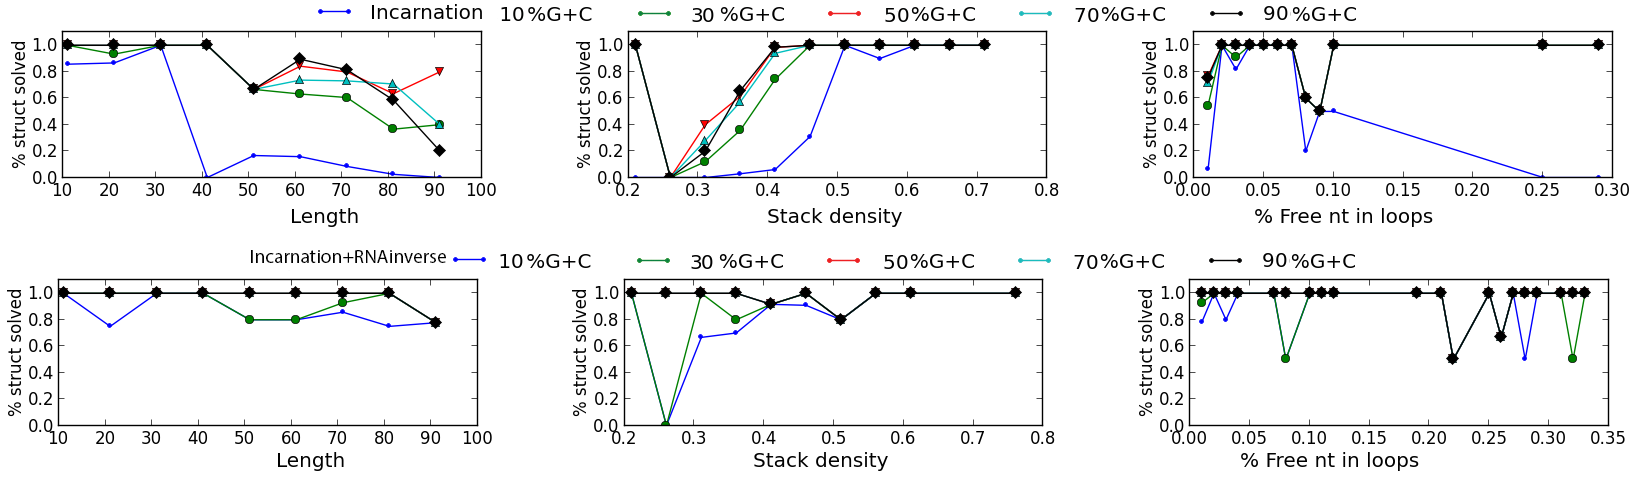
\includegraphics[width=\textwidth]{Figures/struct_solved_vsrnainverse.png}
  \caption{The first row shows the number of structures for which one generated sequence has the 
  structure as MFE when only using \ourprog. The second row shows when we process \ourprog results with \RNAinverse.}
  \label{fig:nb_sols}
\end{figure*}


\subsection{Benchmark \ourprog vs \RNASSD}
%Using the same dataset of $50$ structures, we generated $100$ samples
%per structure %with \RNAinverse. They yield for most parameters
%a high entropy.
%Table.~\ref{tab:nb_rnainv} contains the number of samples with a given \GCContent generated
%with  \RNAinverse, \INFORNA, \NUPACK and \frankenstein. They have a highly concentrated distribution of \GC content showing one of theirs major deficiencies. We present in Fig.~\ref{fig:gcdist} those distributions.

%\begin{figure}[ht]
%  \begin{center}
%    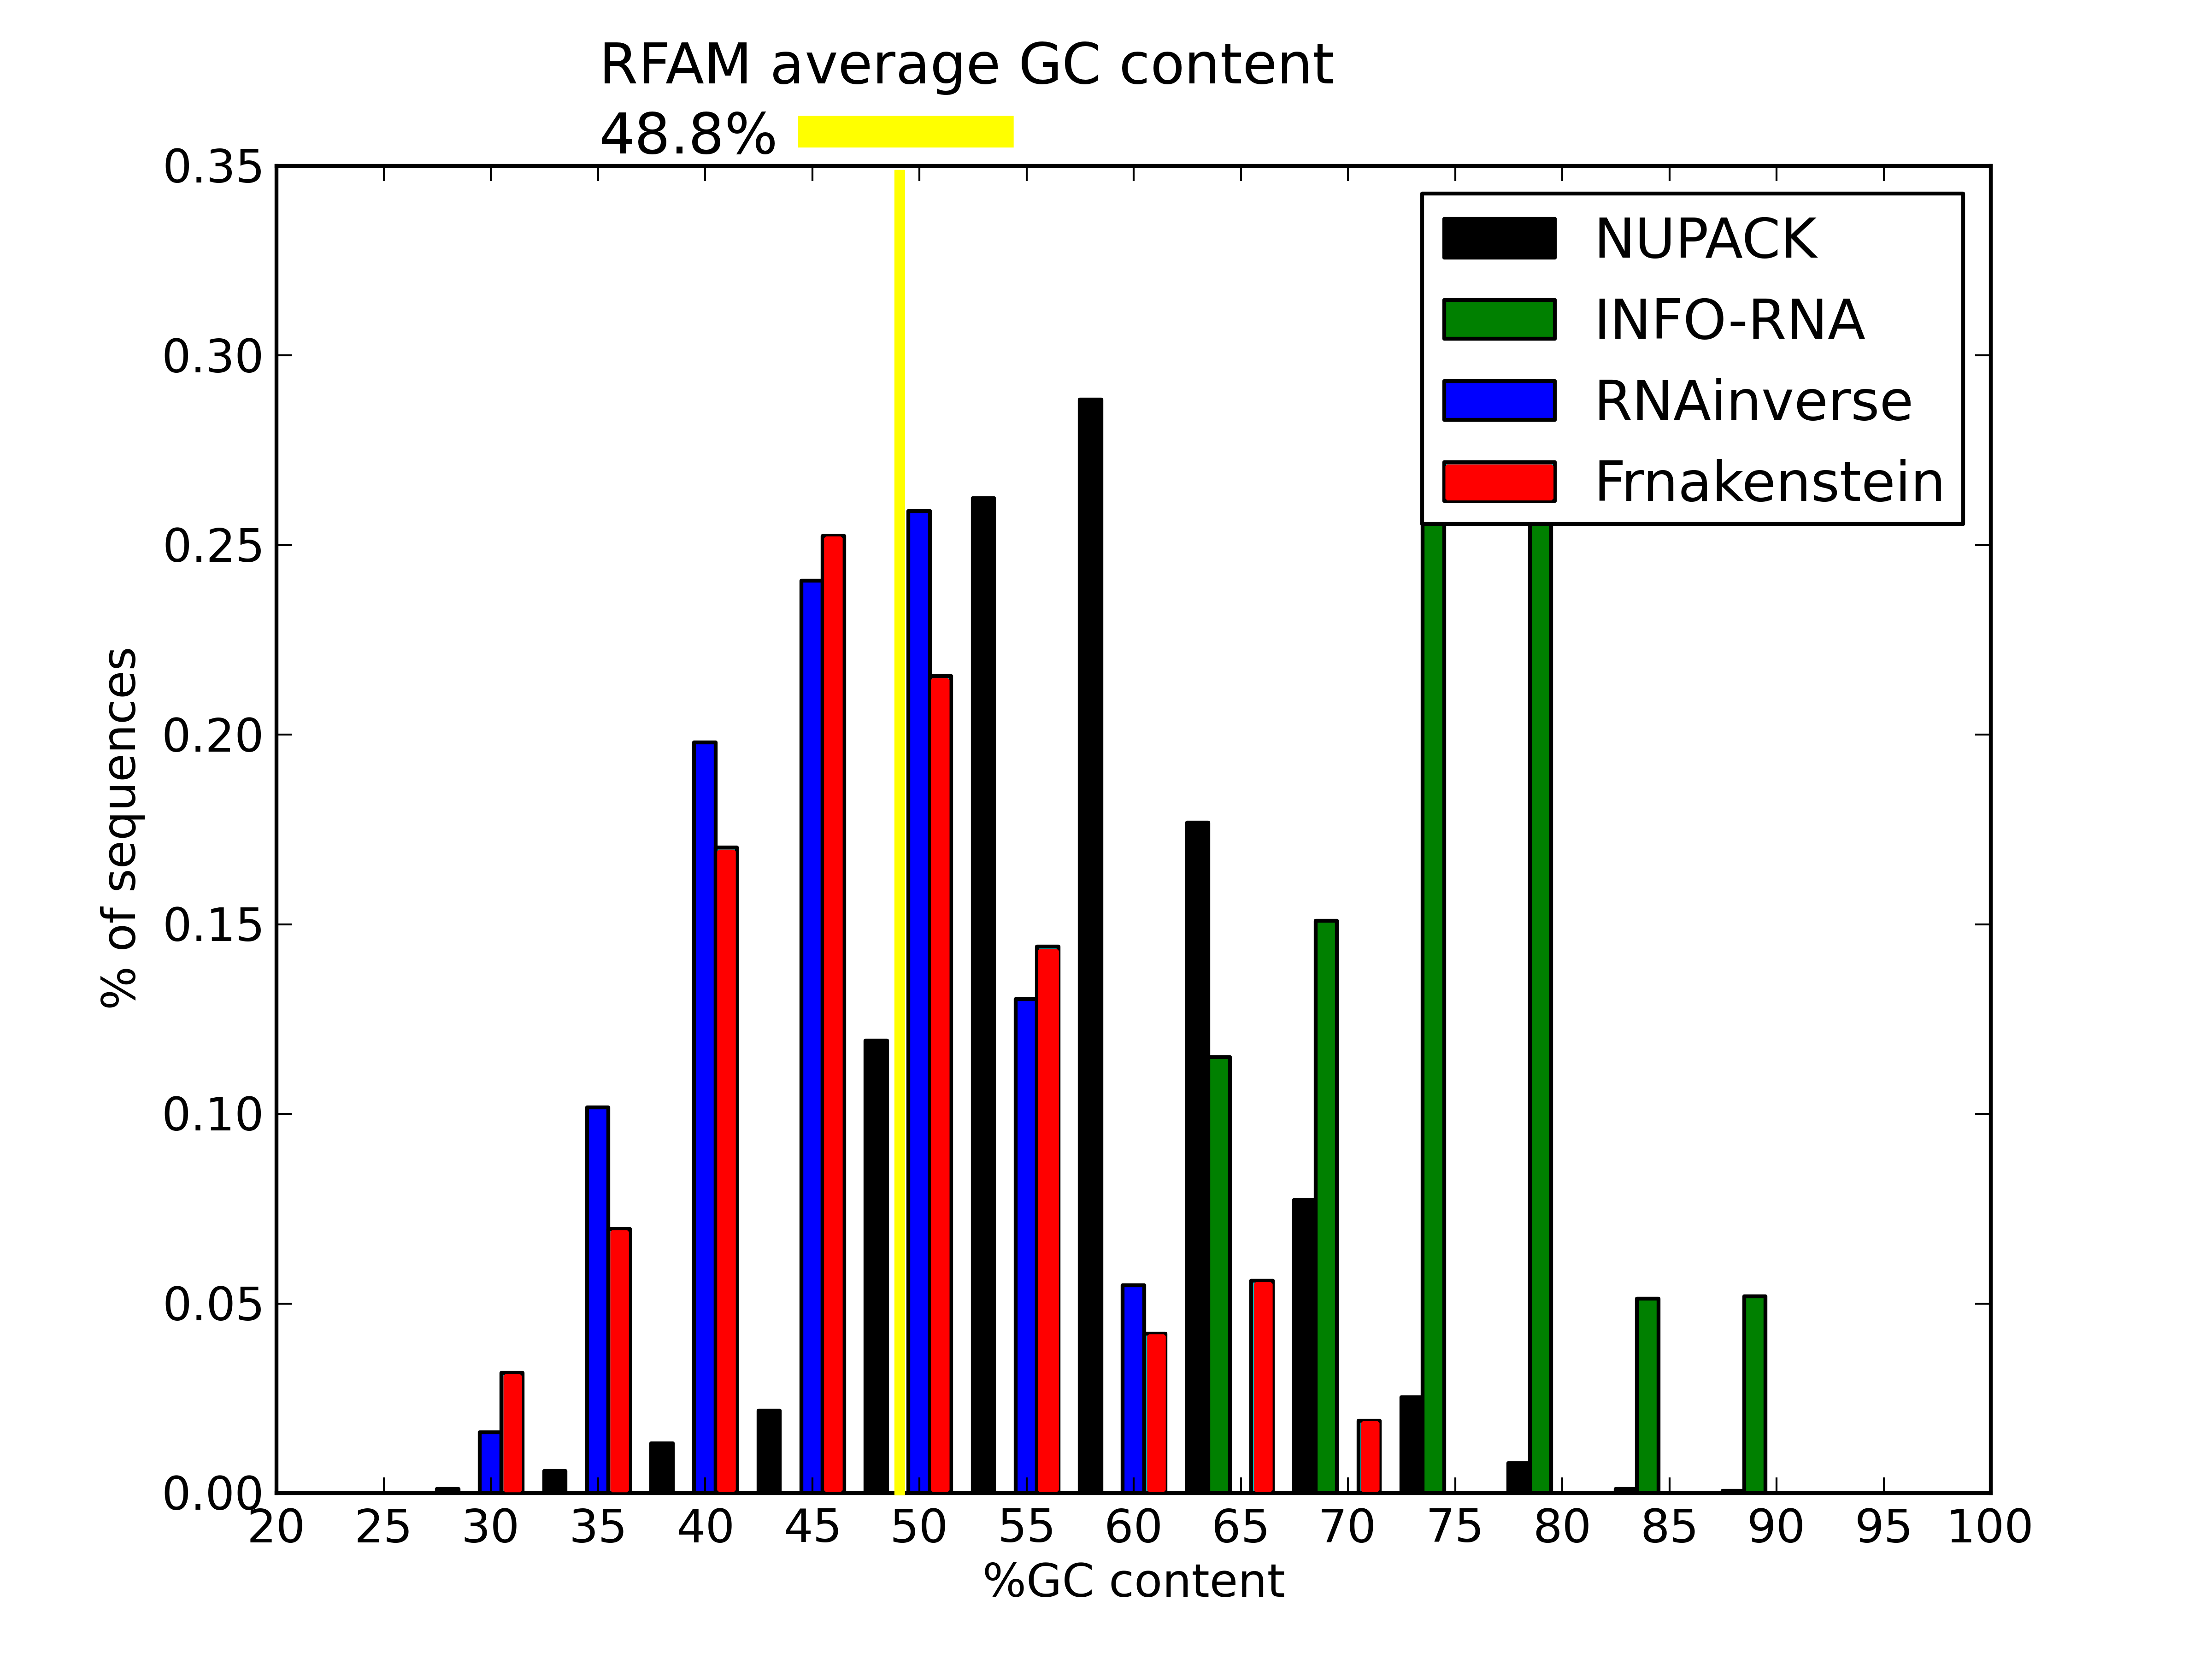
\includegraphics[width=0.5\textwidth]{Figures/histograme_5_gc_distribution_nornaexinv.png}
%  \end{center}
%  \caption{Overall \GCContent distribution for sequences designed using \RNAinverse, \INFORNA, \NUPACK and \frankenstein folding in the desired structure.}
%  \label{fig:gcdist}
%\end{figure}

 For all structures that have been solved 
by the three methods, only \RNASSD, only \texttt{Incarnation} and
\texttt{Incarnation} followed by \RNAinverse, 
we present for different concentration of \GCContent the average sequence identity in Figure.~\ref{fig:identity_50_70_90}
%the average sample entropy and the average base pairs entropy in Figure.~\ref{fig:rnainverse}.

\begin{figure*}[ht!]
  \centering
  \includegraphics[width=\textwidth]{Figures/seq_identity_50_70_90.png}
  \caption{Sequence identity by average \GCContent of $50$, $70$ and $90\%$ for \ourprog,\ourprog+\RNAinverse and \RNASSD.}
  \label{fig:identity_50_70_90}
\end{figure*}
%\begin{table}[h!]
%	\begin{center}
%		\begin{tabular}{|c|ccccc|}
%		\hline
%		Target \GCContent & 10 & 30 & 50 & 70 & 90\\ \hline
%   $\#$\RNAinverse samples& 11 & 437 & 3362 & 1155 & 35\\ \hline
%		\end{tabular}
%	\end{center}
%  \caption{Overall \GCContent distribution for sequences designed using \RNAinverse.}
%	\label{tab:nb_rnainv}
%\end{table}




%\begin{figure*}[ht!]
%	\centering
	%\hspace{-5em}
%	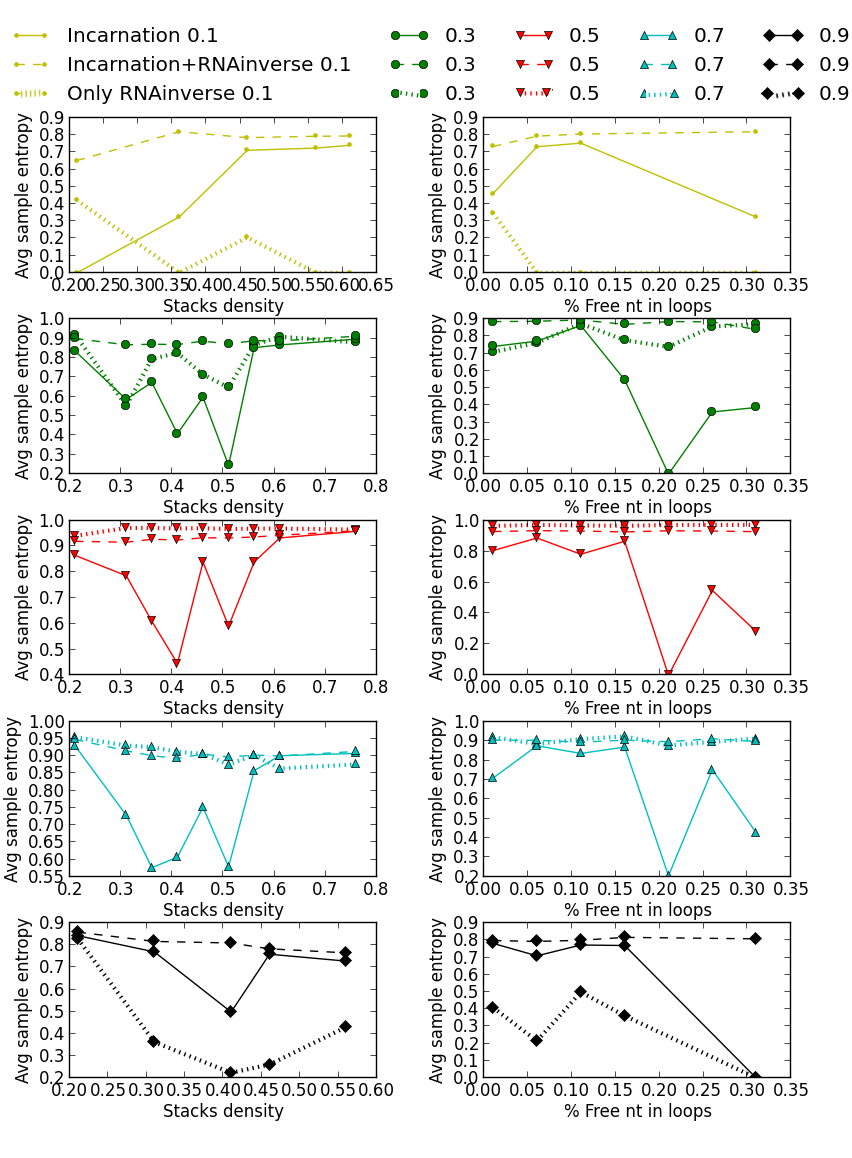
\includegraphics[width=0.5\textwidth]{Figures/RNAinverse_data_100.png}
%	\caption{Entropy and \GCContent  for structures solved by
%	the 3 methods.}
%	\label{fig:rnainverse}
%\end{figure*}
%{\em Récupérer Base-pair entropy}


%The same analysis but only for structures solved by \texttt{Incarnation}
%and \texttt{Incarnation} followed by \RNAinverse, is presented in 
%Fig.~\ref{fig:inc_rnainv}
%
%\begin{figure}
%	\centering
%	\includegraphics{}
%	\caption{Entropy and \texttt{C+G} content for structures solved by
%	the \texttt{Incarnation} and \texttt{Incarnation}$+$\RNAinverse.}
%	\label{fig:inc_rnainv}
%\end{figure}

\subsection{Limited impact on \GC of local-search postprocessing of \ourprog output}
Since local search approaches tend to experience a bias towards \GC{}-rich regions, it could be expected that our glocal approach, by postprocessing unpaired regions using a local search algorithm, would suffer from such a drift.
However, as summarized in Table~\ref{table:impact_on_gc}, we observed that the local search heuristic used to design nucleotides in loop regions has a very limited impact on the \GCContent. For each class of \GCContent, we reported the observed \GCContent in the sequence initially generated by \ourprog, and the observed \GCContent after the \RNAinverse postprocessing (as defined in Section \ref{subsec:glocal_method}). Our results show that the \GCContent is relatively well conserved (less than 6\% variation), with a general tendency of the postprocessing step to bring the \GCContent back to 50\%. 

\begin{table}[h!]
\begin{center}
\resizebox{0.5\textwidth}{!}{
\begin{tabular}{|c|c|c|}
\hline
\multirow{3}{*}{Target \GCContent (\%)}& \multicolumn{2}{c|}{\GCContent (\%) of designed sequences}\\ \cline{2-3}
 & \ourprog & \ourprog + \RNAinverse\\
 & (Global) & ({Glocal}) \\
\hline
10\% & 15\% & 21\% \quad $\nearrow 6\%$\\
30\% & 30\% & 33\% \quad $\nearrow 3\%$\\
50\% & 48\% & 49\% \quad $\nearrow 1\%$\\
70\% & 71\% & 69\% \quad $\searrow 2\%$\\
90\% & 83\% & 78\% \quad $\searrow 5\%$\\
\hline
\end{tabular}
}
\end{center}
\caption{Observed \GCContent of solutions returned by \ourprog (2nd column) and after the application of the local search postprocessing (3rd column).}
\label{table:impact_on_gc}
\end{table}


\end{document}  
